\documentclass[a4paper, 12pt, french, twoside]{article}
\usepackage{graphicx,wrapfig,lipsum}
\usepackage{graphicx}
\usepackage{mathtools}
\usepackage{amsmath}
%\frenchbsetup{StandardLists=true} à inclure si on utilise 
\usepackage[french]{babel}
\usepackage{enumitem}
\usepackage{float}
\usepackage{fontawesome}
%\usepackage[top=2.5cm, bottom=2cm, left=2cm, right=2cm, showframe]{geometry}
\usepackage[top=2.5cm, bottom=2cm, left=2cm, right=2cm]{geometry}
\usepackage{caption}
\usepackage{amsmath}
\usepackage{graphicx} % Required for inserting images
\usepackage{subcaption}
\usepackage{hyperref}
\usepackage{makecell}
\usepackage{amsfonts}
\usepackage{amsthm}


\newtheorem{theorem}{Théorème}[section]
\newtheorem{corollary}{Corollaire}[theorem]
\newtheorem{lemma}[theorem]{Lemme}
\newtheorem{proposition}{Proposition}[theorem]
\newtheorem{defi}{Définition}[theorem]
\newtheorem{rem}{Remarque}[theorem]

\usepackage{pdfpages} % lien Pdf test
 \usepackage{tcolorbox}
\usepackage{multicol}
\usepackage{cleveref}
\crefrangelabelformat{equation}{(#3#1#4--#5#2#6)}
\crefname{equation}{Eq.}{Eqs.}
\Crefname{equation}{Equation}{Equations}


%\usepackage{movie15}
\usepackage{epstopdf}
\usepackage{subcaption}
\usepackage{multicol}

%a abréviations
\def \be {\begin{equation}}
\def \ee {\end{equation}}
\def \dd  {{\rm d}}
\def \bm {\begin{pmatrix}}
\def \em {\end{pmatrix}}

%Ensembles 
\newcommand{\Cc}{{\mathbb{C}}}
\newcommand{\Ct}{\Cc^\times}
\newcommand{\Hh}{{\mathbb{H}}}
\newcommand{\Nn}{{\mathbb{N}}}
\newcommand{\Zz}{{\mathbb{Z}}}
\newcommand{\Zzn}{\Zz/n\Zz}
\newcommand{\ZzNt}{(\Zz/N\Zz)^\times}%quotient 
\newcommand{\Rr}{{\mathbb{R}}}
\newcommand{\Rt}{{\Rr^\times}}
\newcommand{\Qt}{{\Qq^\times}}
\newcommand{\Qq}{{\mathbb{Q}}}
%to do later
\newcommand{\later}[1]{\textcolor{orange}{[#1]}}
\newcommand{\com}[1]{\textcolor{magenta}{[#1]}}

%to make hyper refs not surrounded with red
\hypersetup{pdfborder=0 0 0}
\hypersetup{
    colorlinks=true,
    linkcolor=blue,
    filecolor=magenta,      
    urlcolor=cyan,
    pdftitle={Overleaf Example},
    pdfpagemode=FullScreen,
    }
    
\title{Série 2}

\begin{document}

\maketitle
% \section{Exo (Gaétan)}
% Montrer par contradiction qu'une suite de Cauchy est bornée
% \section{Exo (Gaétan)}
% Montrer qu'une suite croissante, bornée supérieurement converge.

\section{Limites usuelles}
Dans la pratique, nous utilisons des compositions de limites usuelles pour calculer les limites des suites rapidement. Il faut donc les démontrer, comme tout en mathématiques! Trouver les limites à l'infini des suites suivantes :

\begin{enumerate}
    

    \begin{multicols}{2}
    \item $x_n=n$
    \item $x_n= n^p$, $p>0$
    \item $x_n=n^p$, $p\leq 0$
    \item $x_n= a \cdot n^p$, $a,p\in \Rr$
    \item $x_n= \dfrac{n^p}{n^q}$, $p,q\in \Rr$
    \item $x_n=\dfrac{a_pn^p+a_{p-1}n^{p-1}+...+a_0}{b_qn^q+b_{q-1}n^{q-1}+...+b_0}$, $a_i,b_i\in \Rr$, $a_p$ et $b_q$ non nuls et $p,q \in \Rr^+$
    \end{multicols}
\end{enumerate}
% \section{Limites usuelles avancées}
% Ces limites sont plus ardus à démontrer et nécessite des notions qui ne sont pas enseignées dans ce cours. Donc, cet exercice est facultatif. 
% Montrer les limites suivantes
% \begin{enumerate}
%         \item $\underset{{n\to \infty}}\lim \dfrac{x^n}{n!}$, avec $n!=n\cdot (n-1)\cdot \cdot \cdot 3\cdot 2\cdot 1$
%         \item $\underset{{n\to \infty}}\lim \left(1+\dfrac{1}{n}\right)^k$=1, $k\in \Nn$ fixé
% \end{enumerate}

\section{Sous-suites, Principe des deux gendarmes}

\subsection{Sous-suites}
Commençons par étudier la convergence de la suite suivante:
\begin{equation}
    x_n = sin(\frac{n \pi}{2}) \quad \forall n\in \Nn
\end{equation}

\textbf{a)} Représentez quelques points de la suite sur la Figure \ref{fig:exo2.1a}.\\

\begin{figure}[H]
    \centering
    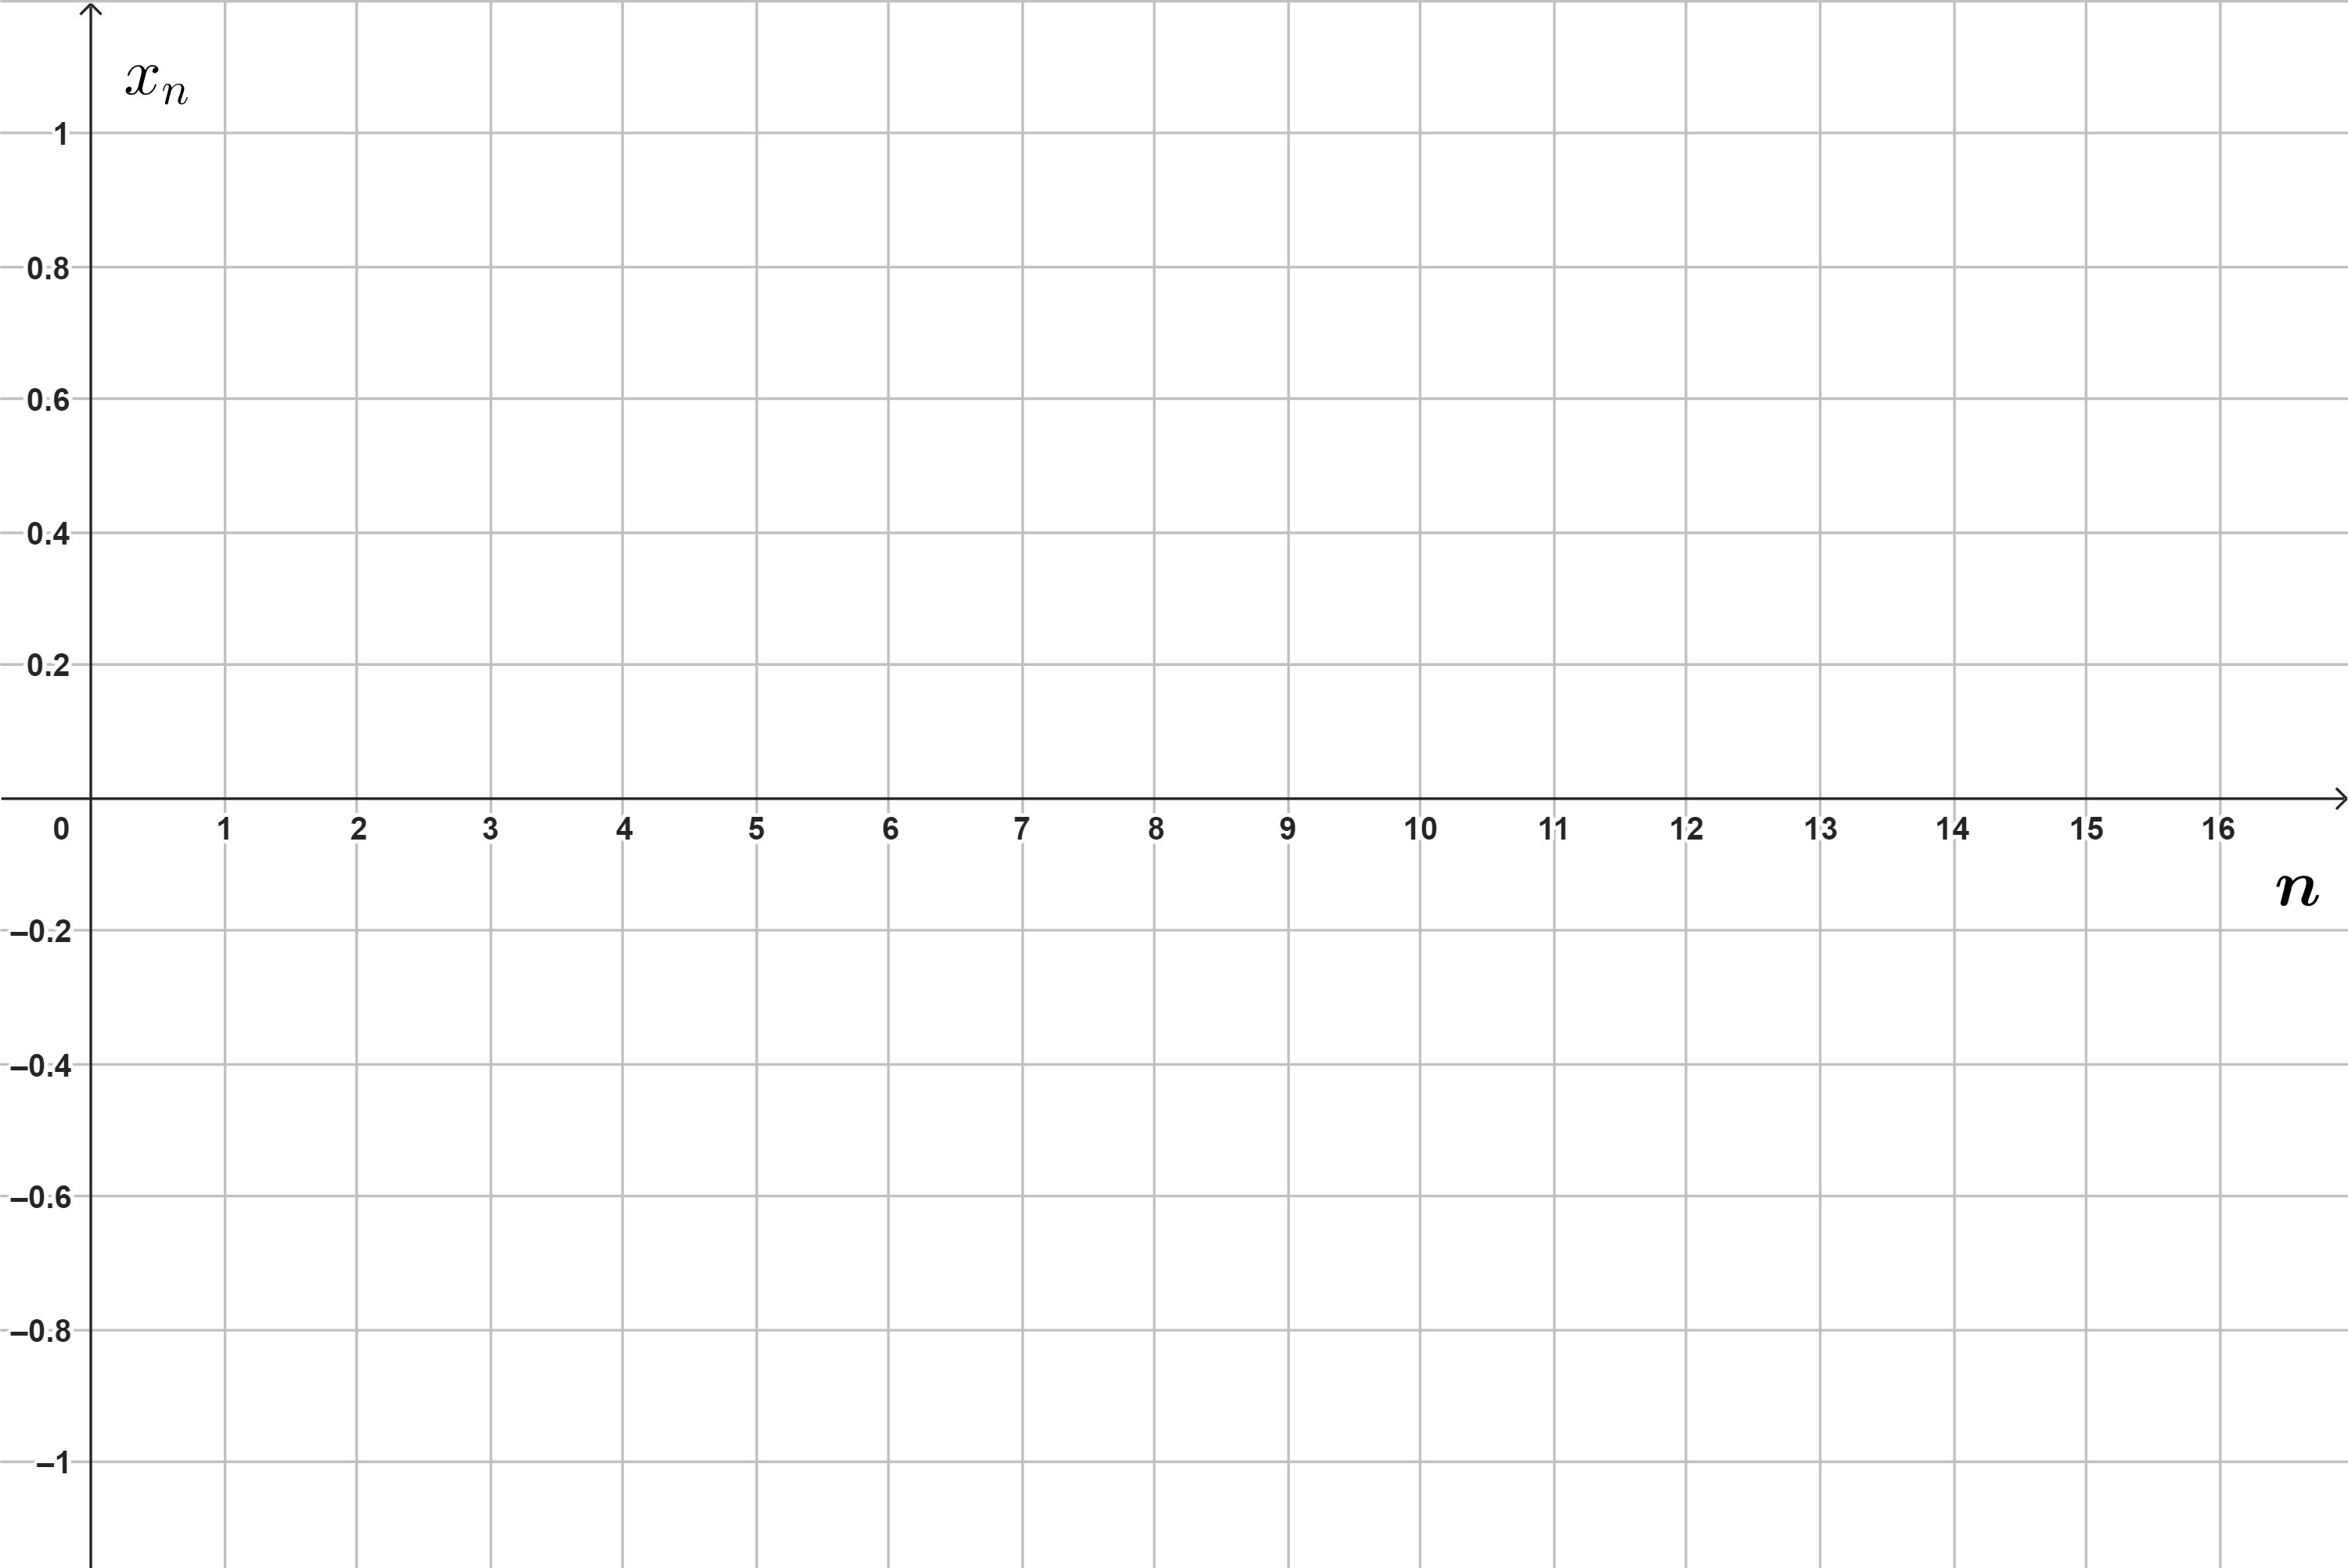
\includegraphics[scale=0.8]{Exercices/exo_sabri.png}
    \caption{Exercice \textbf{2.1 a)}}
    \label{fig:exo2.1a}
\end{figure}

\textbf{b)} Cette suite converge-t-elle? Sinon, pouvez-vous donner une sous-suite qui converge? \\
\textbf{Notez:} Le théorème de Bolzano-Weierstrass nous dit que toute suite bornée admet une sous-suite convergente (elle n'est pas toujours facile à trouver cependant). \\

\textbf{c)} Quelles sont les limites inférieure et supérieure de $x_n$ ? \\

Passons à présent à la suite suivante:
\begin{equation}
    y_n = \frac{1}{n} sin(\frac{n \pi}{2}) \quad \forall n\in \Nn_0
    \label{exo_sous_suite}
\end{equation}

\textbf{d)} Représentez quelques points de cette suite sur la Figure \ref{fig:exo2.1d}. Cette suite converge-t-elle? Sinon, pouvez-vous donner une sous-suite qui converge? \\

\begin{figure}[H]
    \centering
    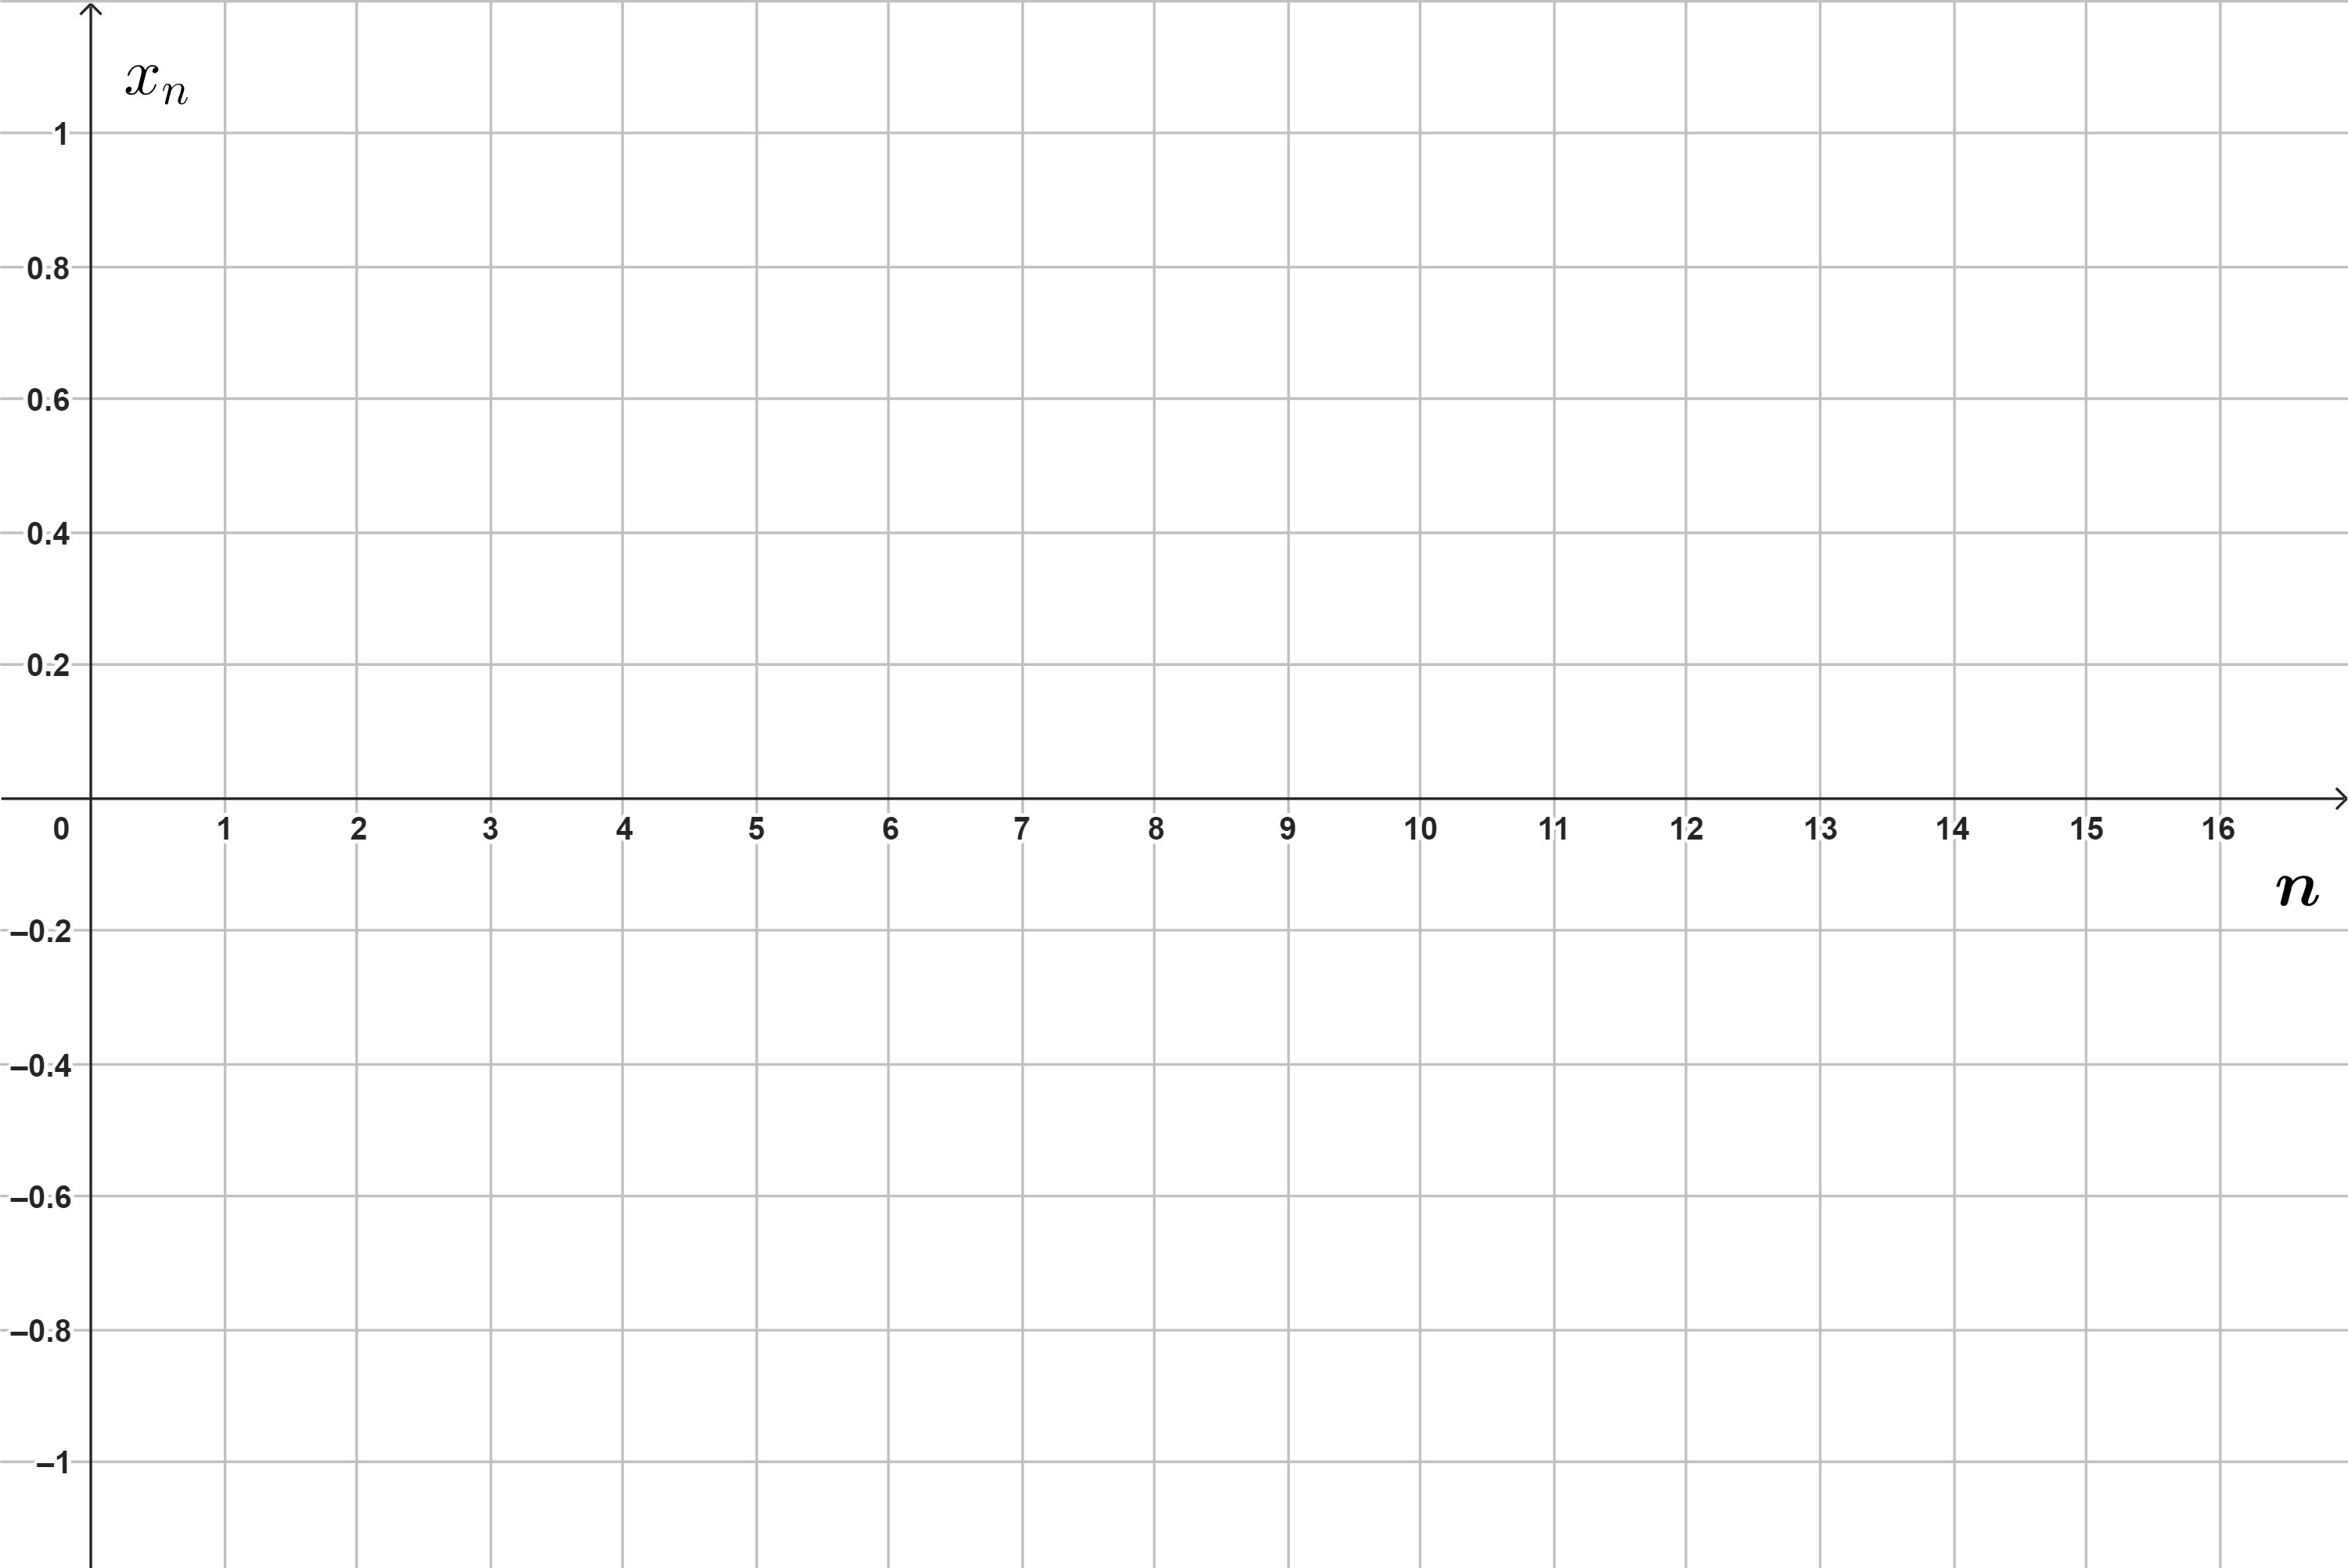
\includegraphics[scale=0.8]{Exercices/exo_sabri.png}
    \caption{Exercice \textbf{2.1 d)}}
    \label{fig:exo2.1d}
\end{figure}\\ \\

\textbf{e)} La sous-suite d'une suite convergente peut-elle converger vers une valeur différente? Si oui, donner un exemple. Sinon, démontrez-le.

\subsection{Principe des deux gendarmes}
En traçant quelques points de la suite \eqref{exo_sous_suite}, on voit clairement qu'elle converge. Montrons-le plus rigoureusement en utilisant le Principe des deux gendarmes.\\

\textbf{a)} Trouvez deux suites $v_n$ et $w_n$ qui convergent vers $0$ et telles que $v_n \leq y_n \leq w_n$. Tracez-les sur la Figure \ref{fig:exo2.1d} afin de vous assurer que les deux gendarmes font bien leur travail. \\

\textbf{b)} Démontrez que la convergence de $v_n$ et $w_n$ implique celle de $y_n$ (en d'autres mots, démontrez le Principe des deux gendarmes, bien sûr sans regarder le polycopié ou vos notes...). \\

\faLightbulbO \quad \fbox{\textbf{Discutez}} Quels ``gendarmes" utiliseriez-vous pour la suite suivante ?
\begin{equation}
    z_n = \frac{1}{n+sin(n)}, \quad n \geq 2
\end{equation}

\section{Suite de Cauchy}
Toute suite réelle converge si et seulement si c'est une suite de Cauchy. Nous allons essayer de mieux comprendre ce qu'est une suite de Cauchy en étudiant l'exemple suivant:
\begin{equation}
    x_n = \frac{(-1)^n}{n} \quad \forall n\in \Nn_0
\end{equation}

\textbf{a)} Montrez que la suite $x_n$ est de Cauchy en utilisant la définition. Aidez-vous de la Figure \ref{fig:exo3a} pour mieux visualiser le problème si nécessaire.\\

\begin{figure}[H]
    \centering
    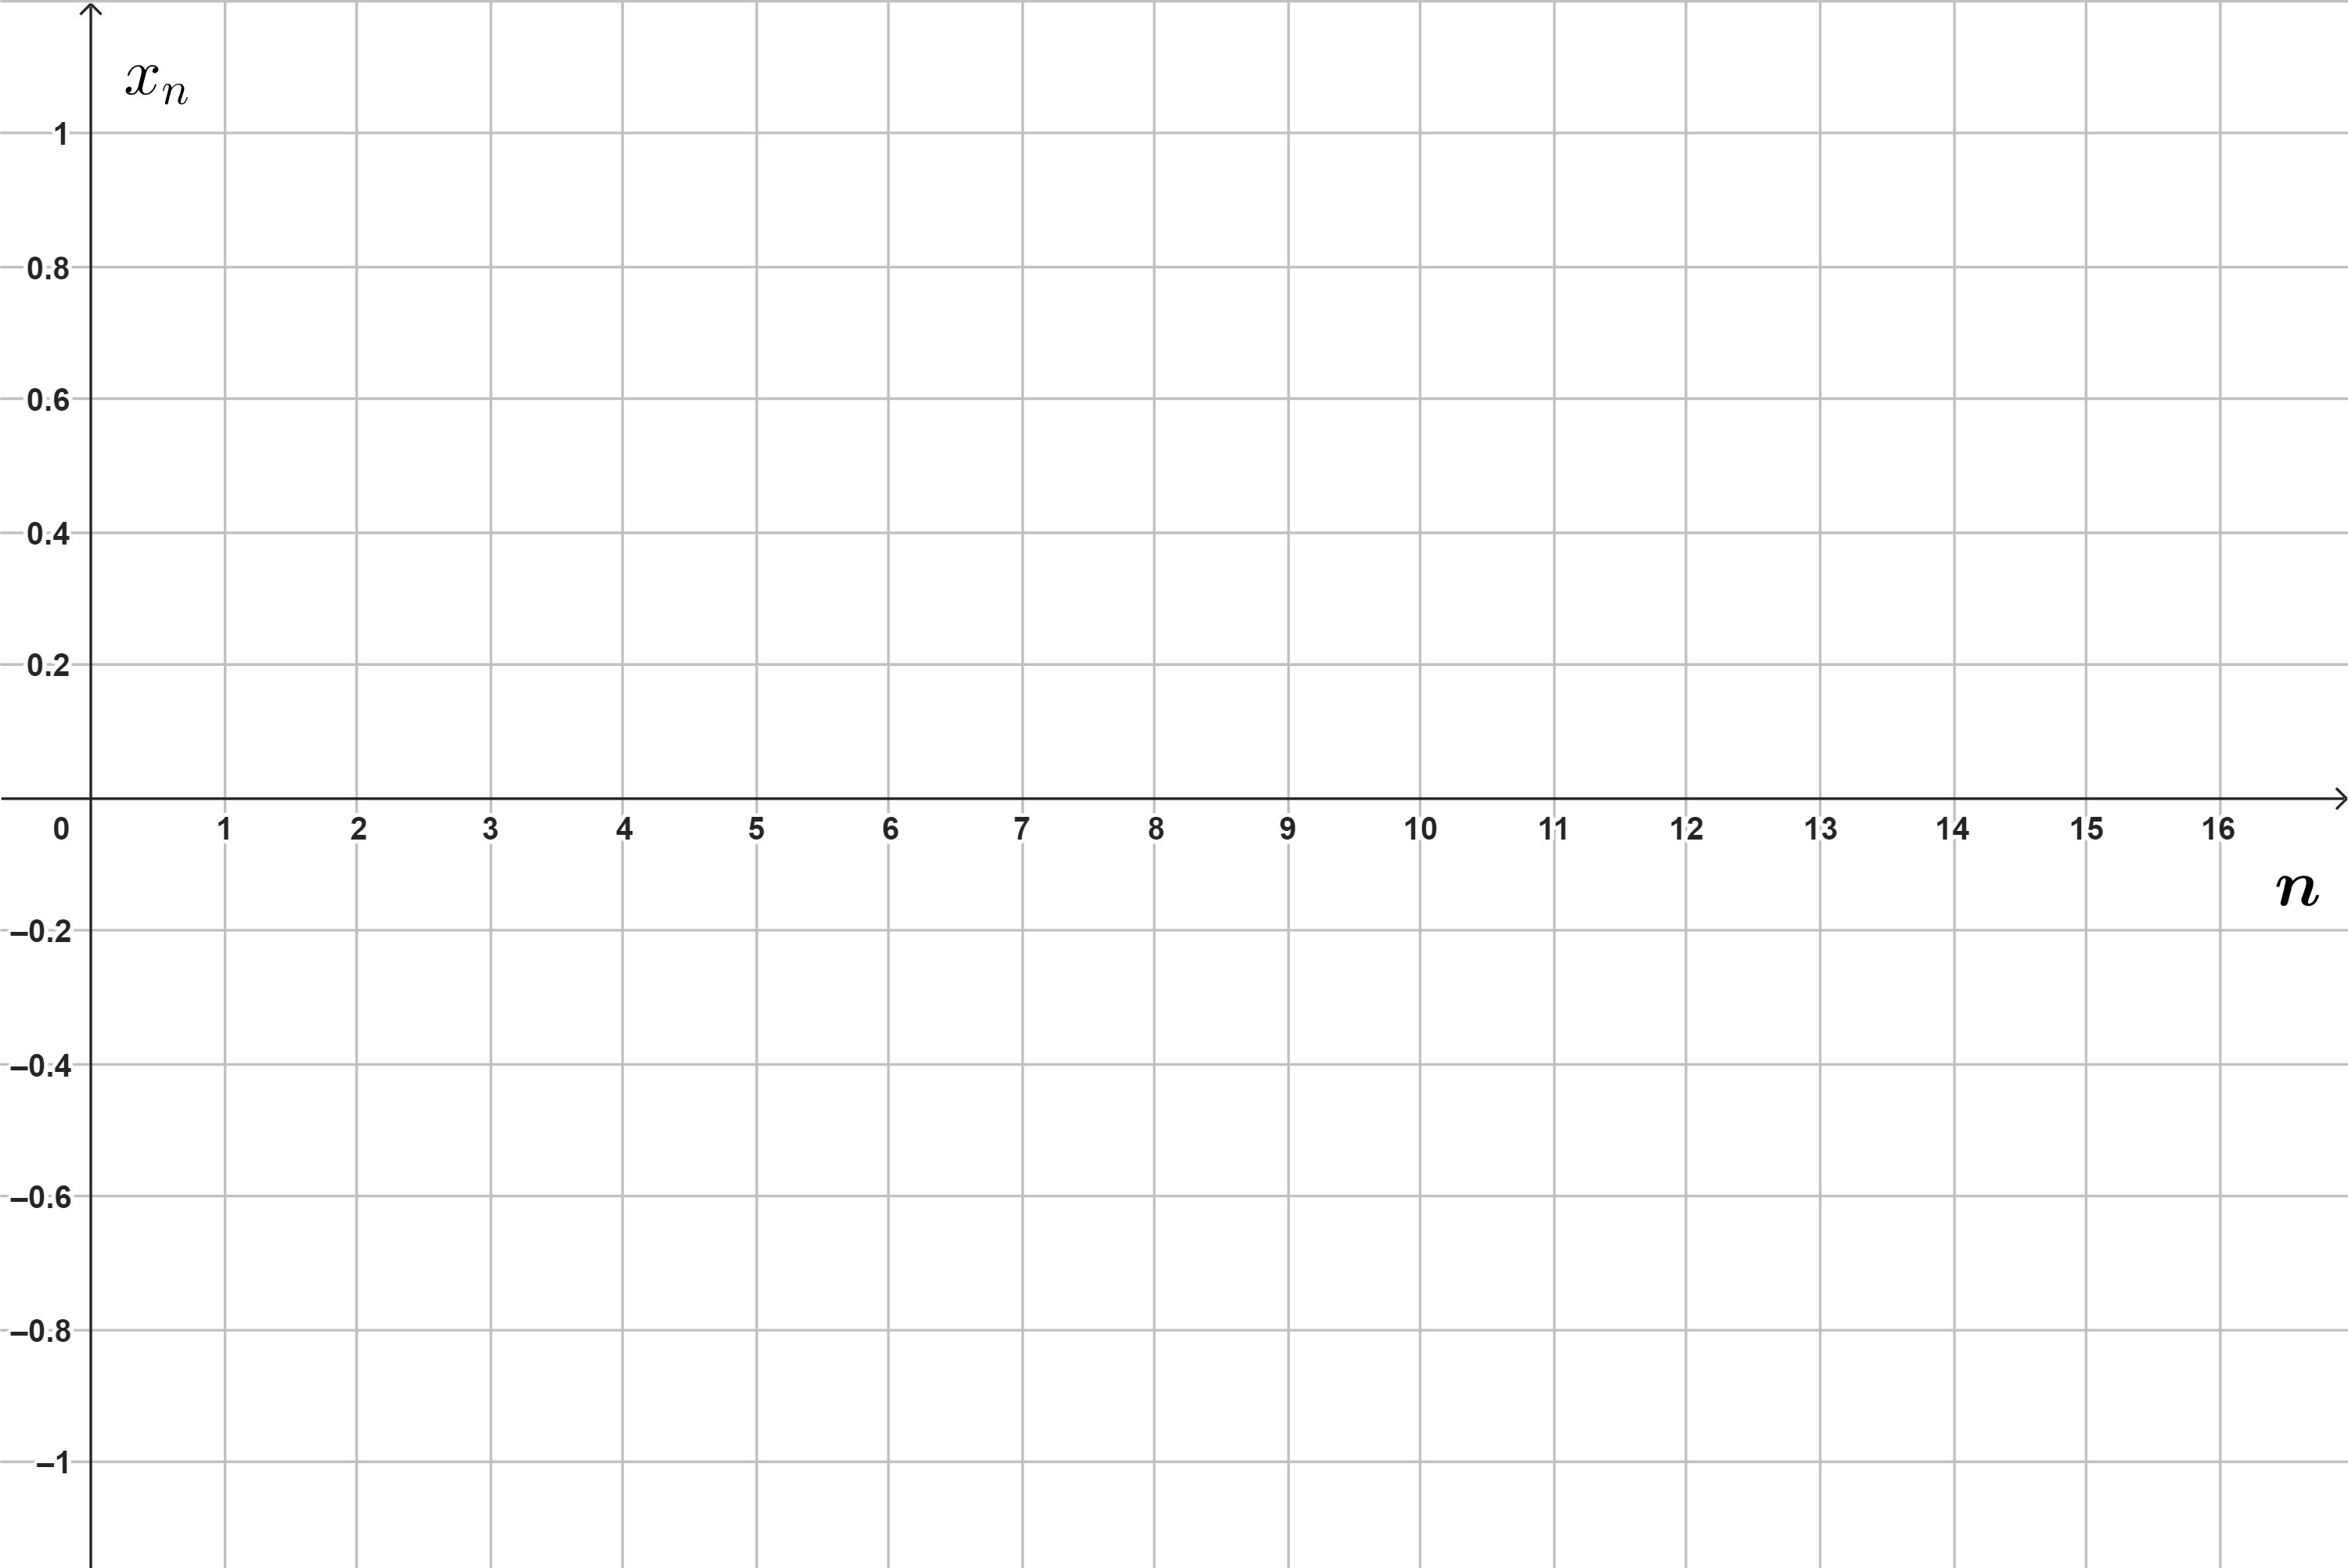
\includegraphics[scale=0.8]{Exercices/exo_sabri.png}
    \caption{Exercice \textbf{3 a)}}
    \label{fig:exo3a}
\end{figure}\\ \\

\textbf{b)} Montrez par contradiction qu'une suite de Cauchy est bornée. \\
\textbf{Indice:} Partez du principe que la suite n'est pas bornée, et montrez que cela contredit la définition de suite de Cauchy. \\

\faLightbulbO \quad \fbox{\textbf{Discutez}} A l'exercice \textbf{b)}, aurait-on pu démontrer la proposition en partant du principe que la suite n'est pas de Cauchy, pour ensuite montrer que cela contredit la suite bornée?




\end{document}